\section{The Basics: Deep Learning}

% Slide 8 - The Core Idea
\begin{frame}{The Core Idea}
    \begin{itemize}
        \item Replace \textbf{hand-engineered features} with \textbf{trainable multilayer networks}
        \item Why this matters: feature engineering was the bottleneck
    \end{itemize}
    
    \vspace{1em}
    % TODO: Add diagram: raw input → layers → output
    \begin{center}
        \texttt{Raw Input → Layer 1 → Layer 2 → ... → Output}
    \end{center}
\end{frame}

% Slide 9 - Meet Geoffrey Hinton
\begin{frame}{Meet Geoffrey Hinton}
    \begin{columns}
        \column{0.4\textwidth}
        % TODO: Add photo
        % 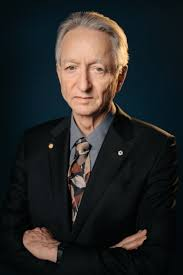
\includegraphics[width=\textwidth]{figures/hinton}
        
        \column{0.6\textwidth}
        \begin{itemize}
            \item Co-author of the \textbf{1986 backpropagation paper}
            \item Invented \textbf{Boltzmann machines} (1985)
            \item \textbf{Nobel Prize in Physics 2024}
        \end{itemize}
    \end{columns}
    
    \vspace{1em}
    \textit{``One of the authors literally helped invent what we're about to explain.''}
\end{frame}

% Slide 10 - Backpropagation
\begin{frame}{Backpropagation}
    % TODO: Add feed-forward network diagram
    
    \begin{enumerate}
        \item \textbf{Forward pass:} Input → through layers → output
        \item \textbf{Compute loss:} How wrong are we?
        \item \textbf{Backward pass:} Propagate gradients back through layers
        \item \textbf{Update weights:} Adjust in direction that reduces error
    \end{enumerate}
    
    \vspace{1em}
    \textbf{ReLU:} Fastest activation function - what the paper recommends
    
    % TODO: Add Python code example here
\end{frame}

% Slide 11 - Stochastic Gradient Descent
\begin{frame}{Stochastic Gradient Descent}
    \begin{itemize}
        \item The optimization engine
        \item Discovered by multiple groups in the 70s and 80s
        \item Including Hinton's group
    \end{itemize}
    
    \vspace{1em}
    \begin{quote}
        ``This simple procedure usually finds a good set of weights surprisingly quickly.''
    \end{quote}
\end{frame}

% Slide 12 - "But Does it Actually Work?"
\begin{frame}{``But Does it Actually Work?''}
    The saddle point rebuttal:
    
    \begin{quote}
        ``The landscape is packed with a combinatorially large number of saddle points where the gradient is zero, and the surface curves up in most dimensions and curves down in the remainder.''
    \end{quote}
    
    \vspace{1em}
    \textbf{Direct answer to the skeptics.}
    
    The authors know exactly what objection you just had.
\end{frame}

% Slide 13 - The 2006 Breakthrough
\begin{frame}{The 2006 Breakthrough}
    \begin{itemize}
        \item \textbf{CIFAR group} - first model to detect features \textit{without labeled data}
        \item Worked around limitations: small datasets, no ReLU, poor GPU support
        \item \textbf{Proved deep learning was worth pursuing}
    \end{itemize}
    
    \vspace{1em}
    \textbf{Reveal:} The authors don't even mention that \textit{they were the ones who did this.}
    
    \vspace{1em}
    Led to first commercial win: \textbf{speech recognition on Android by 2012}
\end{frame}
